\minisec{Parallelität}
On-Chip-Multithreading: Mehrere Threads pro CPU (gegen Pipelinestalling)\\
\textcolor{red}{Beachten: Lücken innerhalb eines Threads (vgl Pause in Abb.)}

Feinkörnig: Abwechselndes Ausführen (Jeden Takt ein anderer Thread); nur 1 Thread pro Takt\\
Grobkörnig: ausführung des Threads bis Leertakt eintritt (evtl. Wechselverzögerung beachten); nur 1 Thread pro Takt\\
Simultan: vgl. Grobkörnig, Threadwechsel innerhalb eines Taktes möglich\\
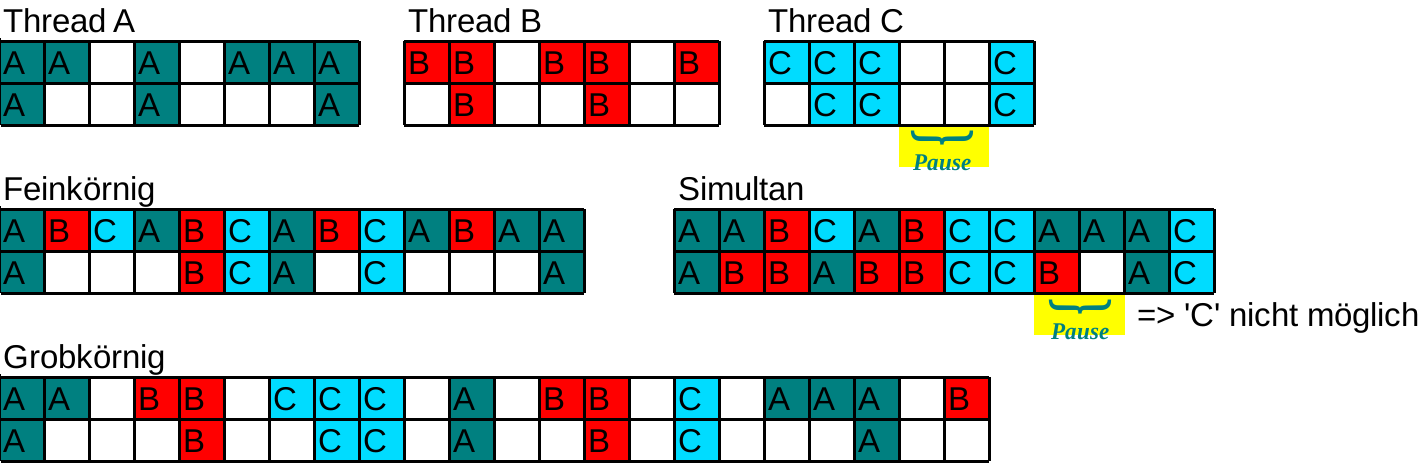
\includegraphics[width=\textwidth]{Multithreading}

